%% SW design: Applikationsmodeller

Selve designet af softwaren bygger på de følgende applikationsmodeller. Her laves der sekvens- og klassediagrammer over hver del af systemet samt klassebeskrivelser hvor funktionen for de enkelte metoder beskrives.

\subsection{Master}
Applikationsmodeller for Master.

\begin{figure}[htbp] \centering
{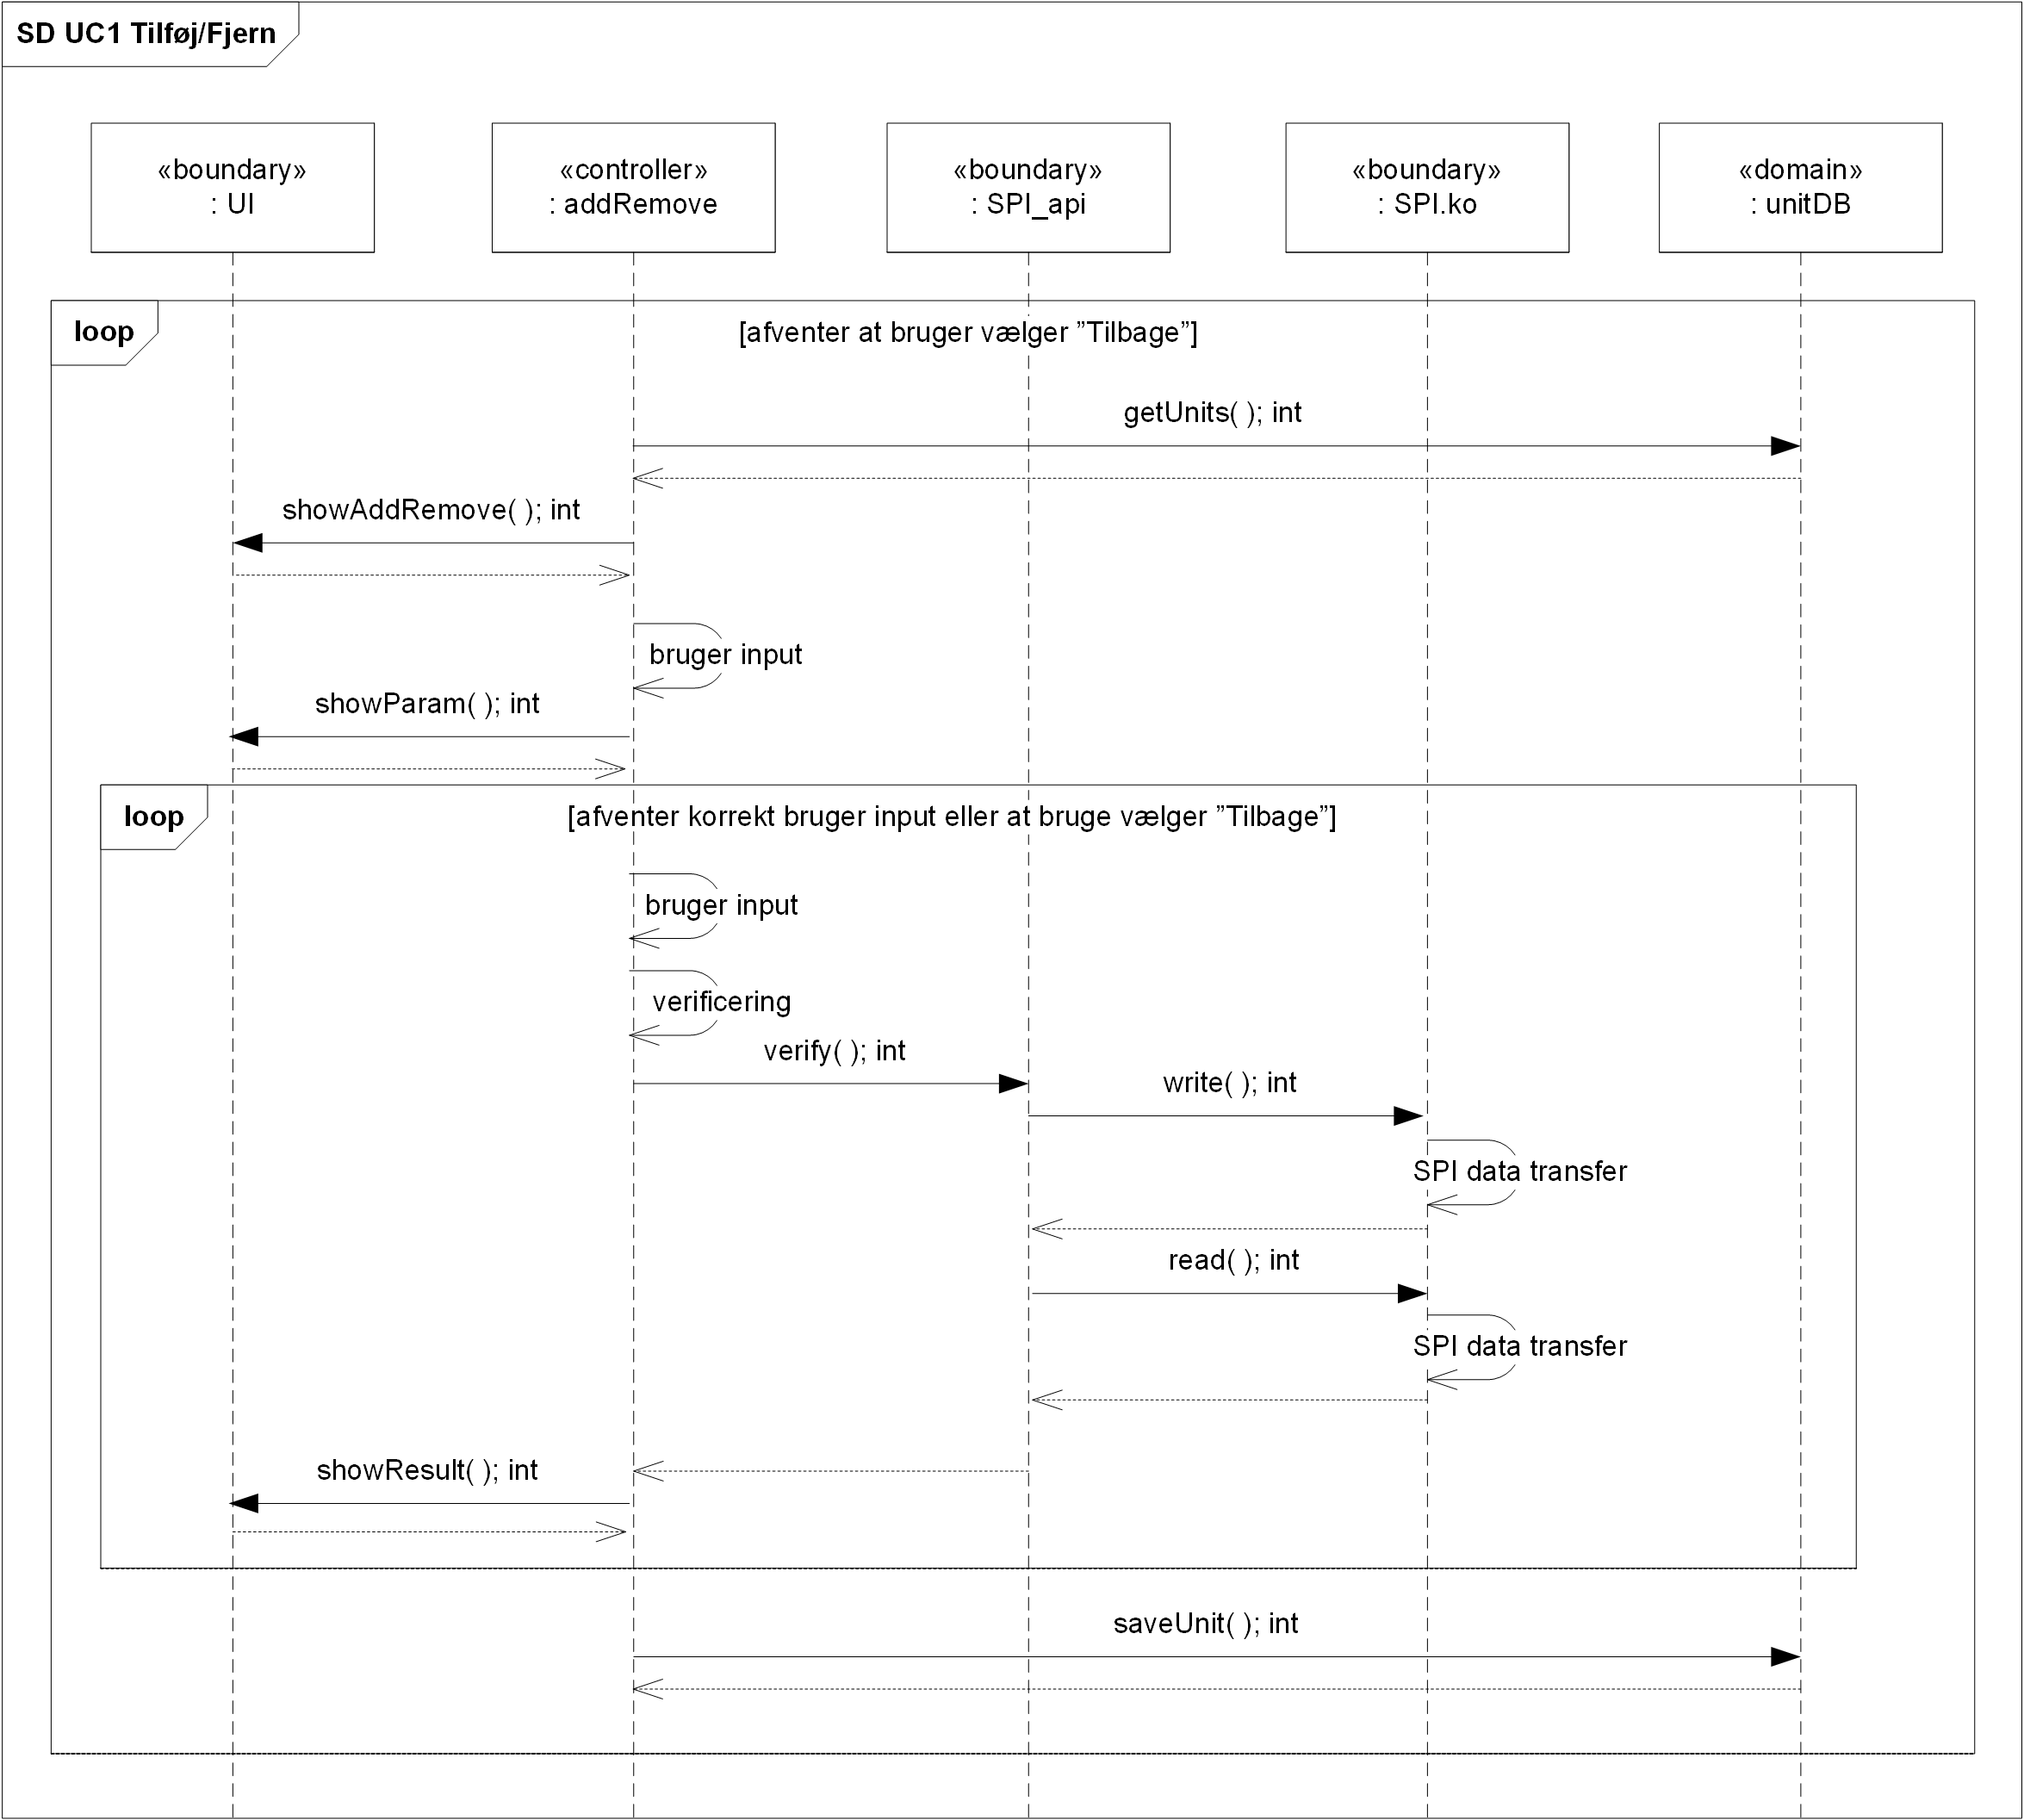
\includegraphics[scale=0.8]{filer/design/a_uc1}}
\caption{Sekvensdiagram UC1}
\label{fig:Sekvensdiagram UC1}
\end{figure} 

\begin{figure}[htbp] \centering
{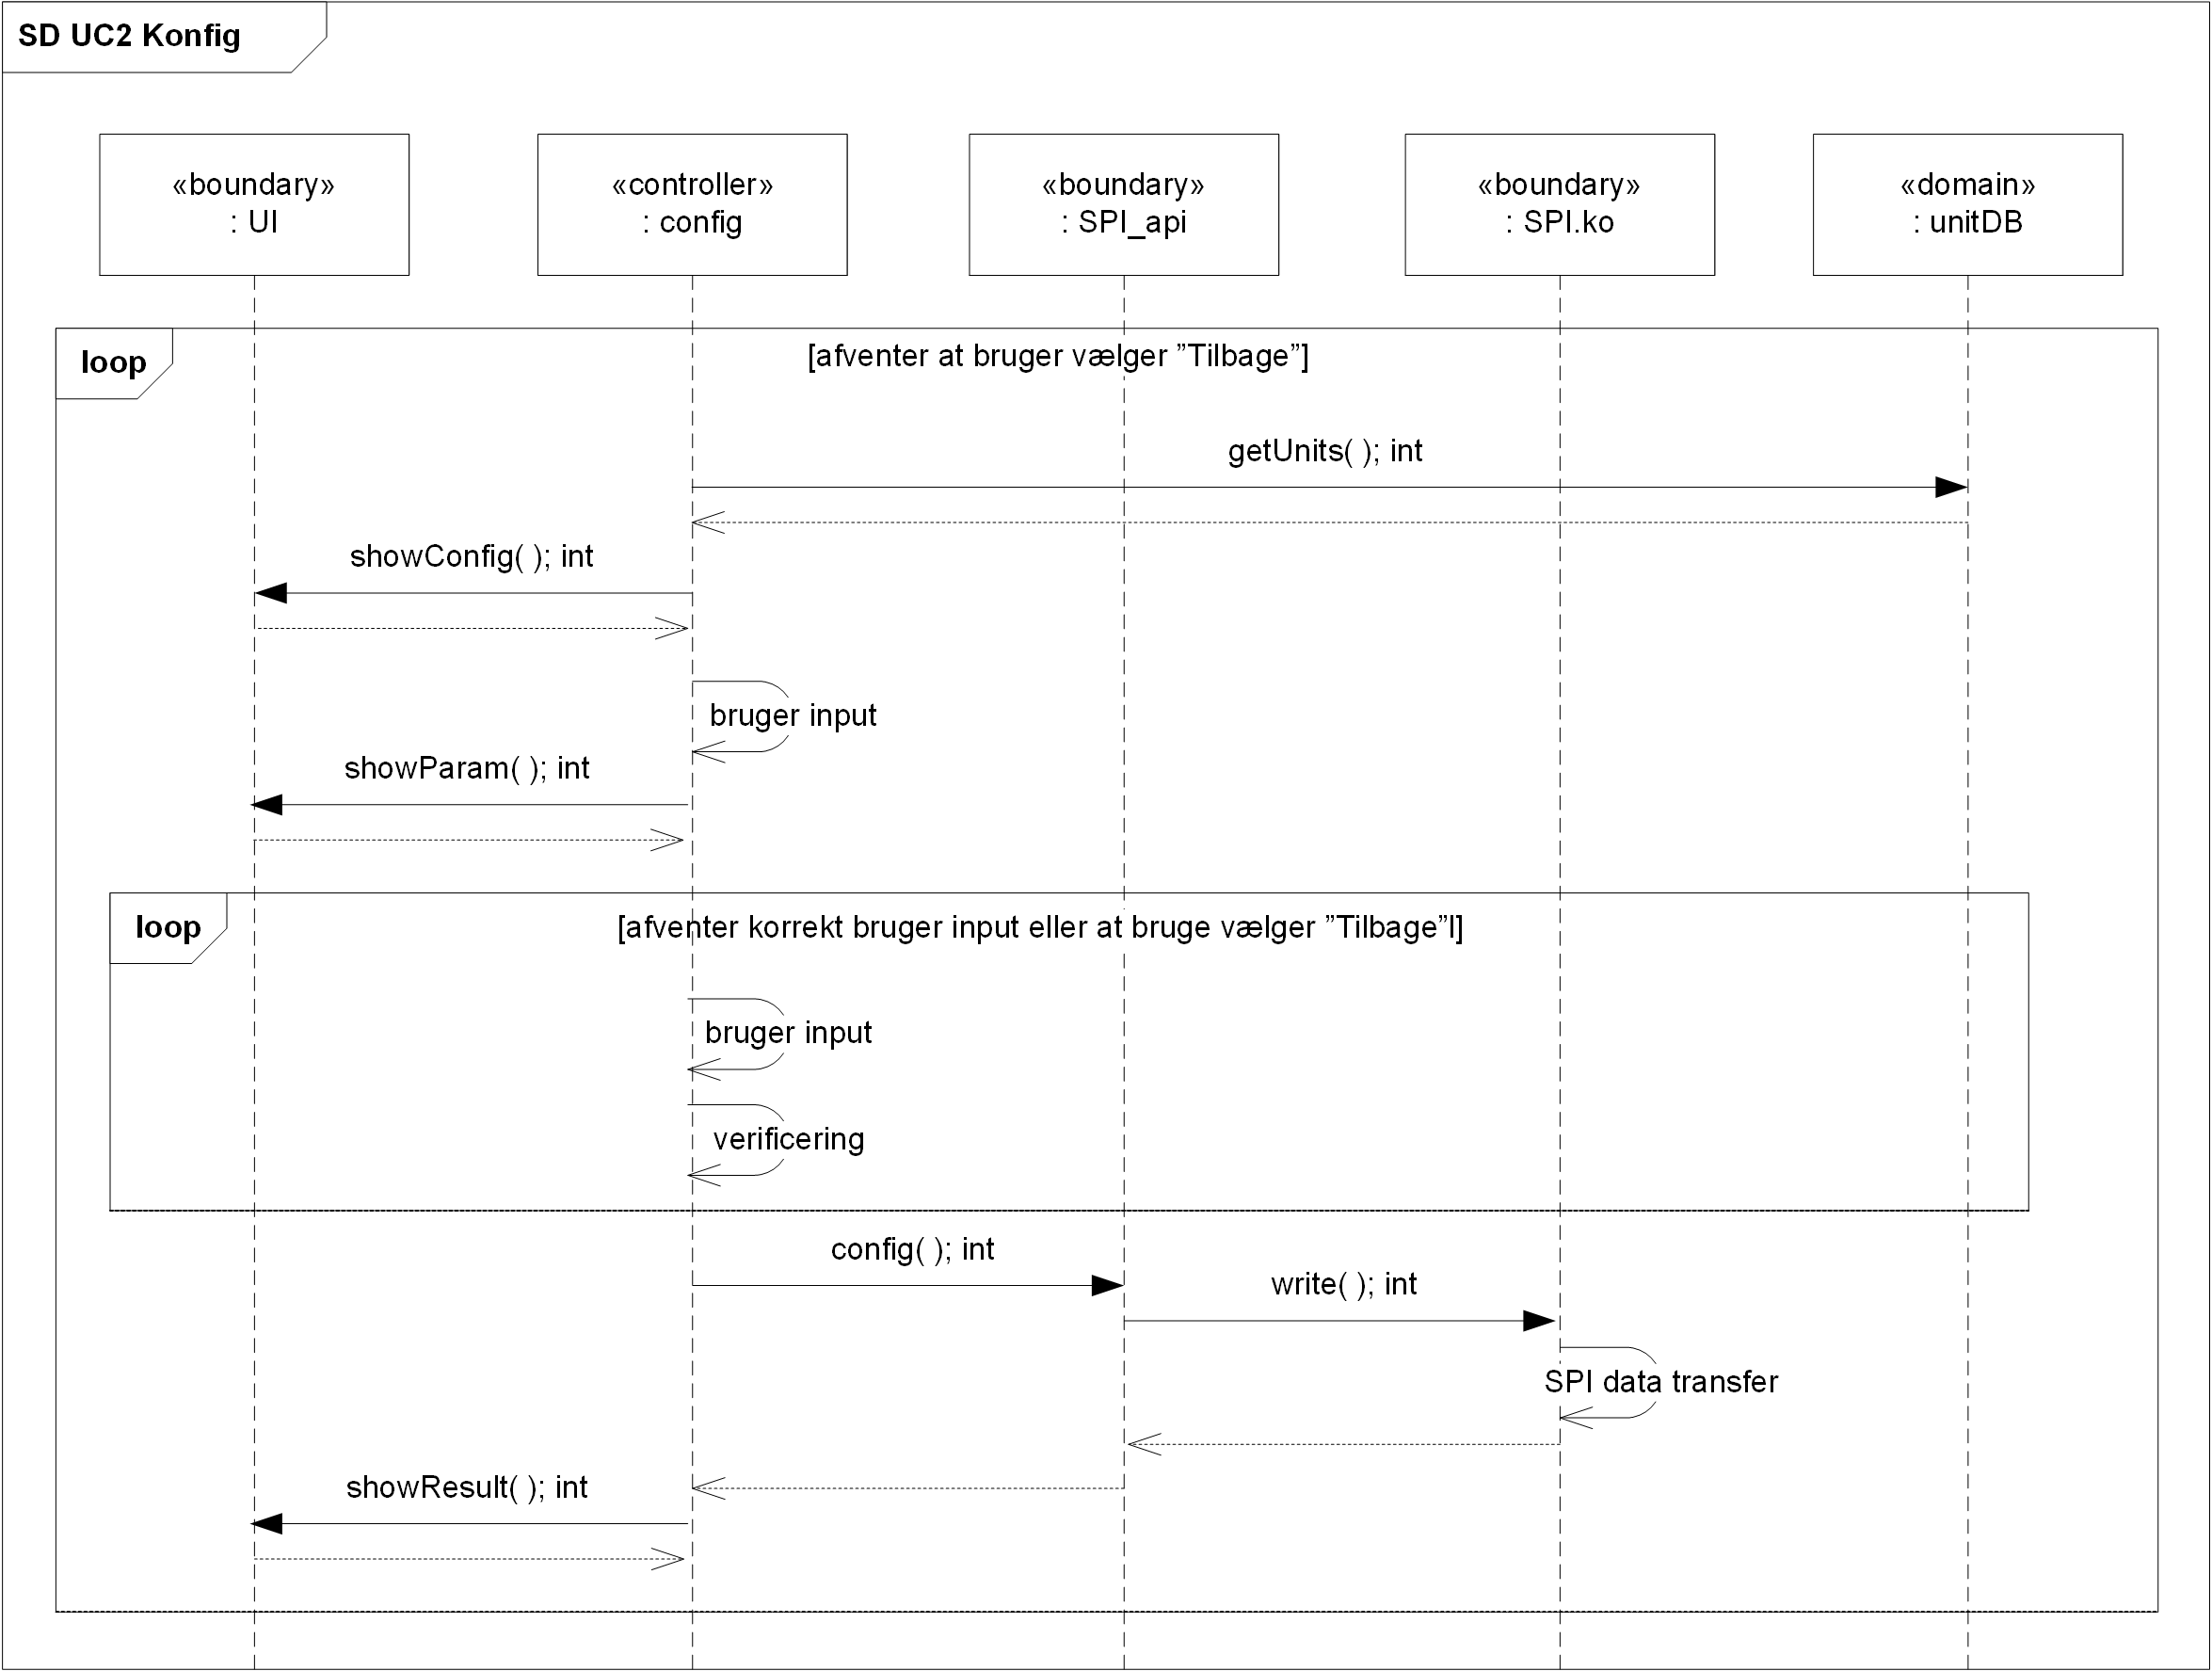
\includegraphics[scale=0.8]{filer/design/a_uc2}}
\caption{Sekvensdiagram UC2}
\label{fig:Sekvensdiagram UC2}
\end{figure} 

\begin{figure}[htbp] \centering
{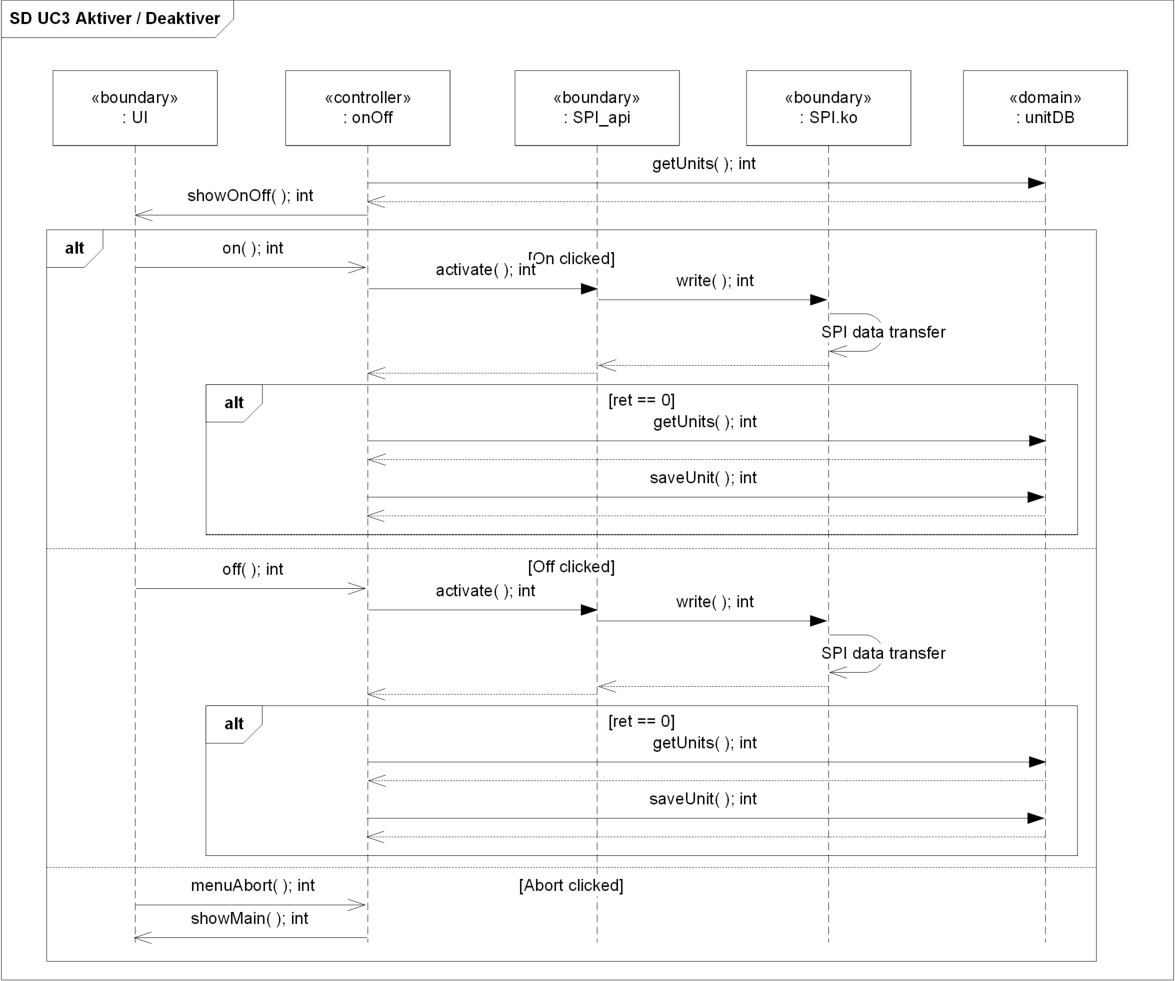
\includegraphics[scale=0.8]{filer/design/a_uc3}}
\caption{Sekvensdiagram UC3}
\label{fig:Sekvensdiagram UC3}
\end{figure} 

\begin{figure}[htbp] \centering
{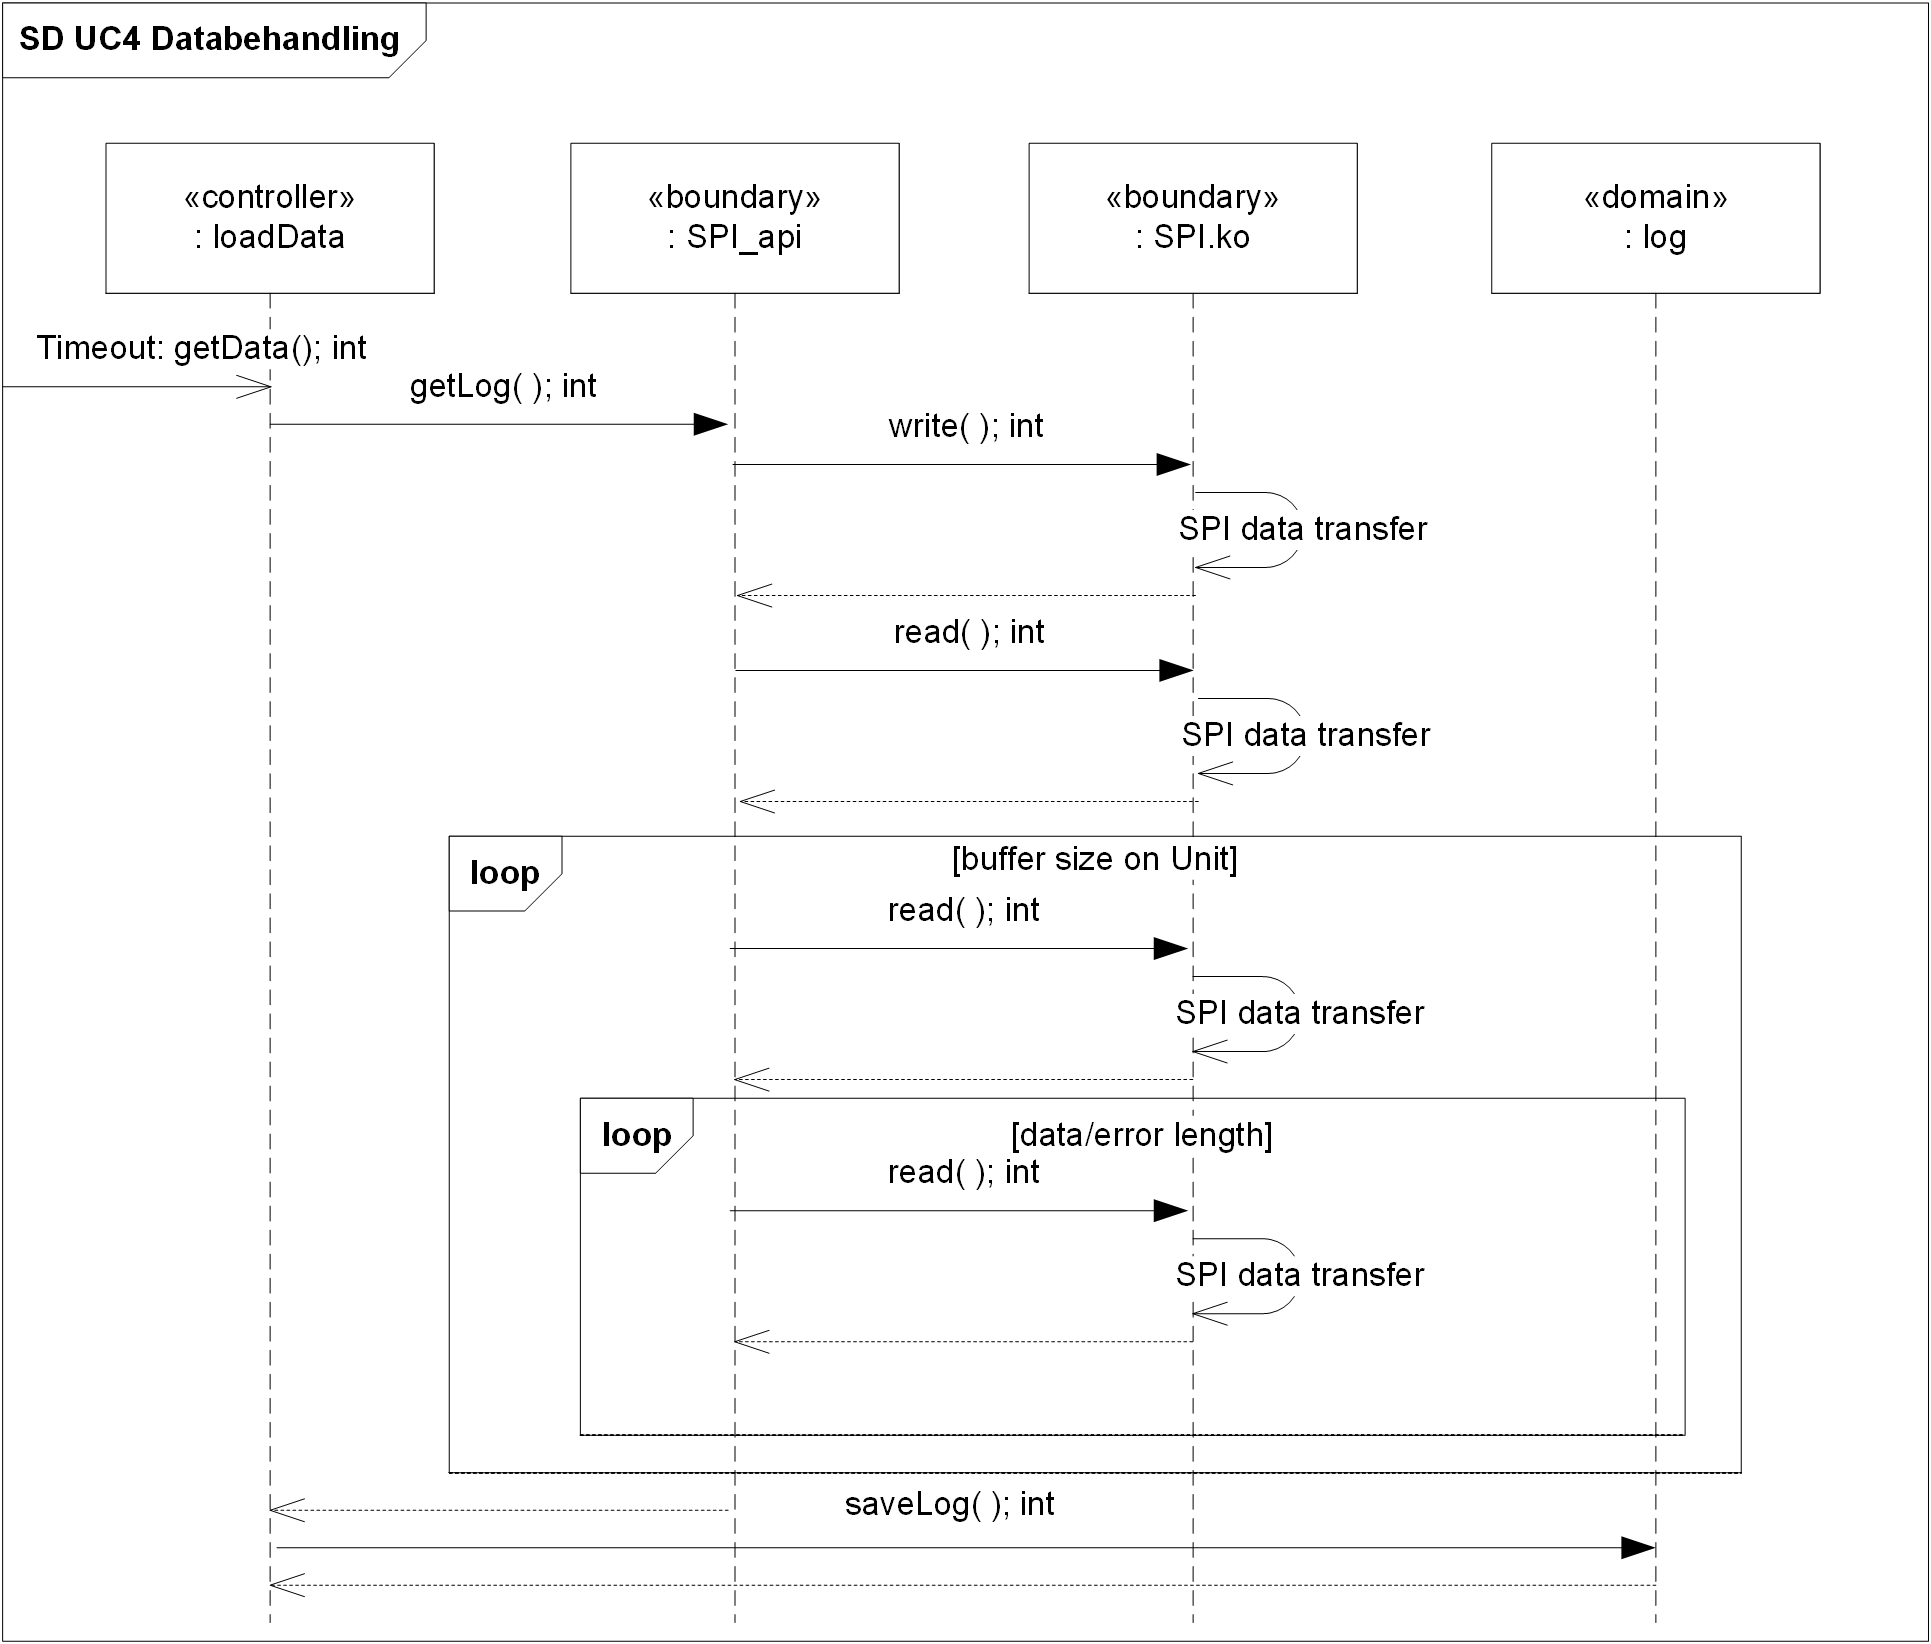
\includegraphics[scale=0.8]{filer/design/a_uc4}}
\caption{Sekvensdiagram UC4}
\label{fig:Sekvensdiagram UC4}
\end{figure} 

\begin{figure}[htbp] \centering
{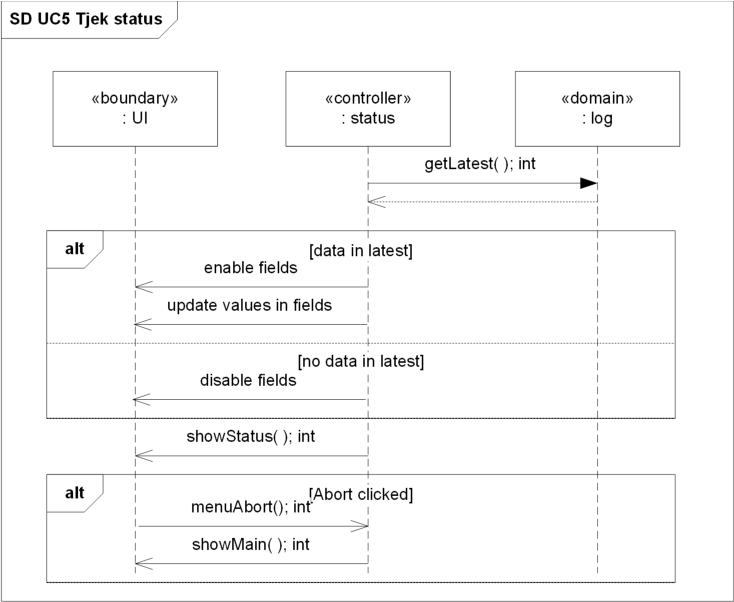
\includegraphics[scale=1]{filer/design/a_uc5}}
\caption{Sekvensdiagram UC5}
\label{fig:Sekvensdiagram UC5}
\end{figure} 

\begin{figure}[htbp] \centering
{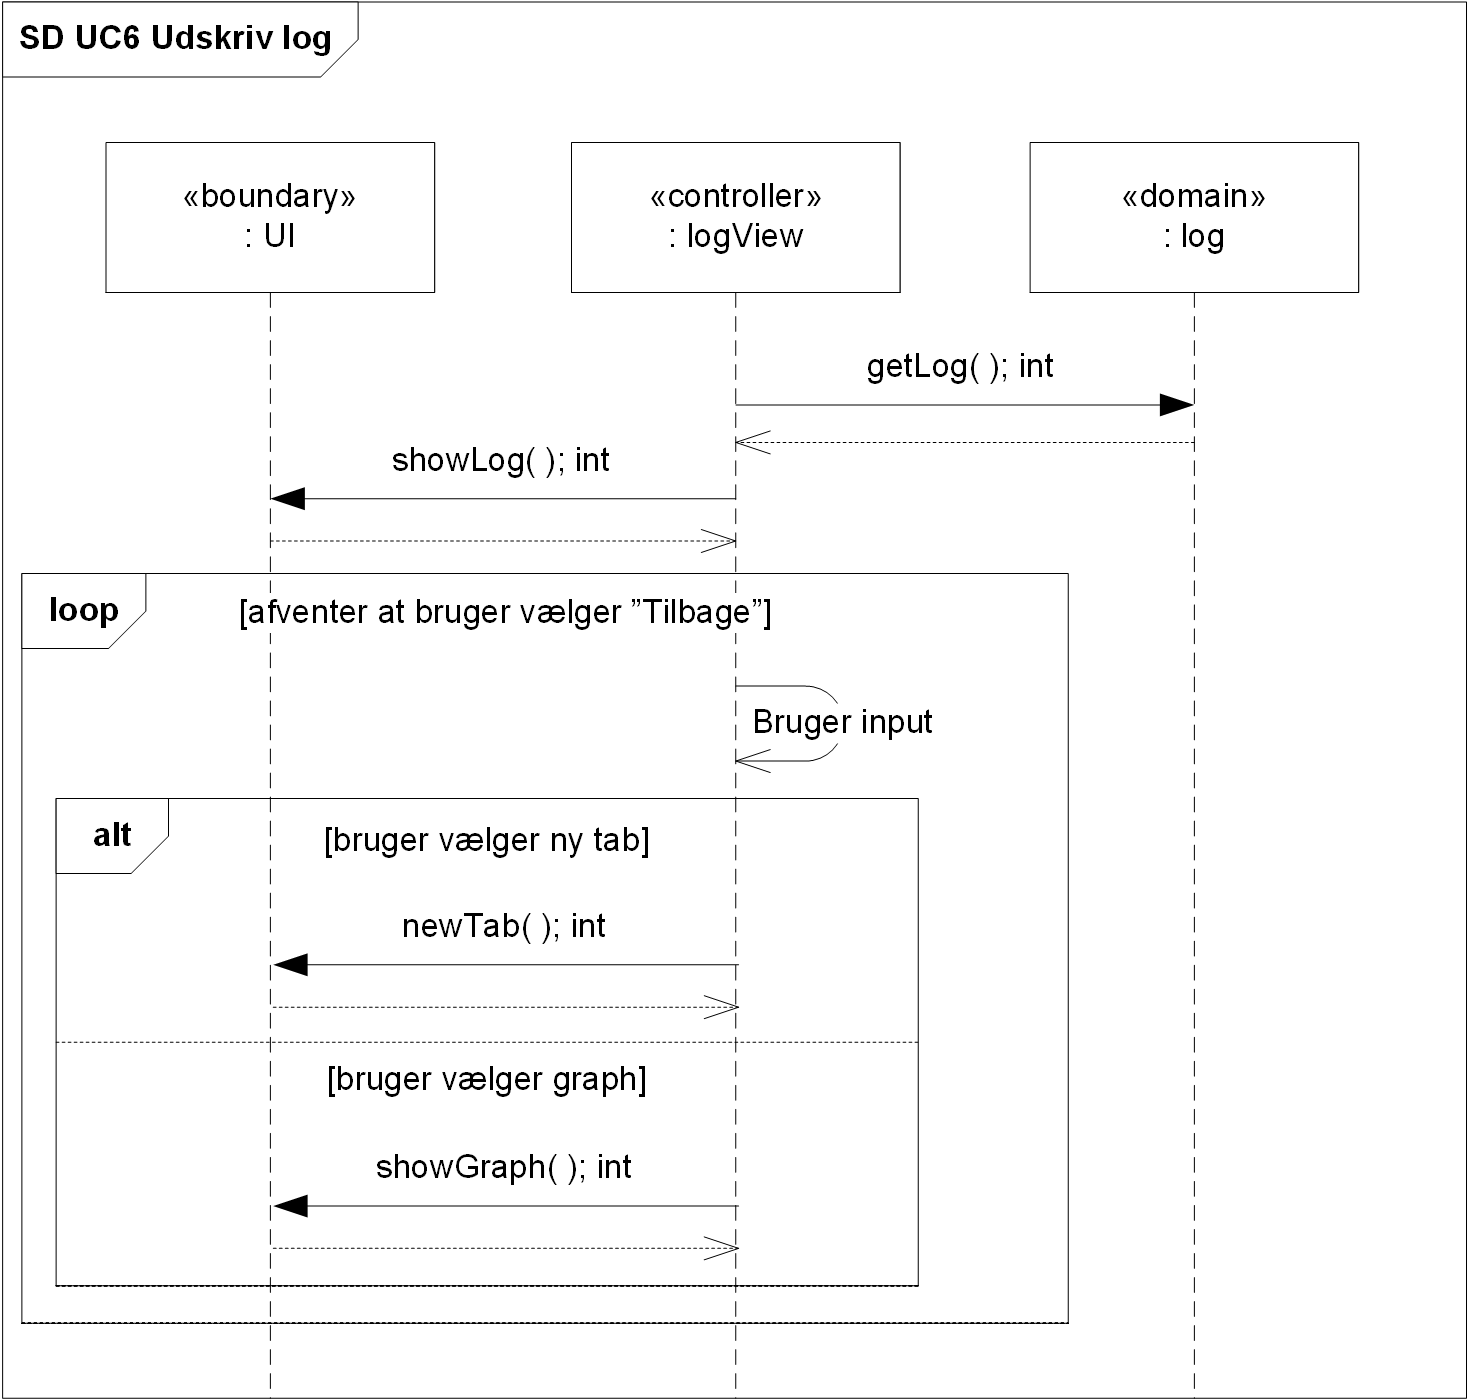
\includegraphics[scale=1]{filer/design/a_uc6}}
\caption{Sekvensdiagram UC6}
\label{fig:Sekvensdiagram UC6}
\end{figure} 

\clearpage
\begin{figure}[htbp] \centering
{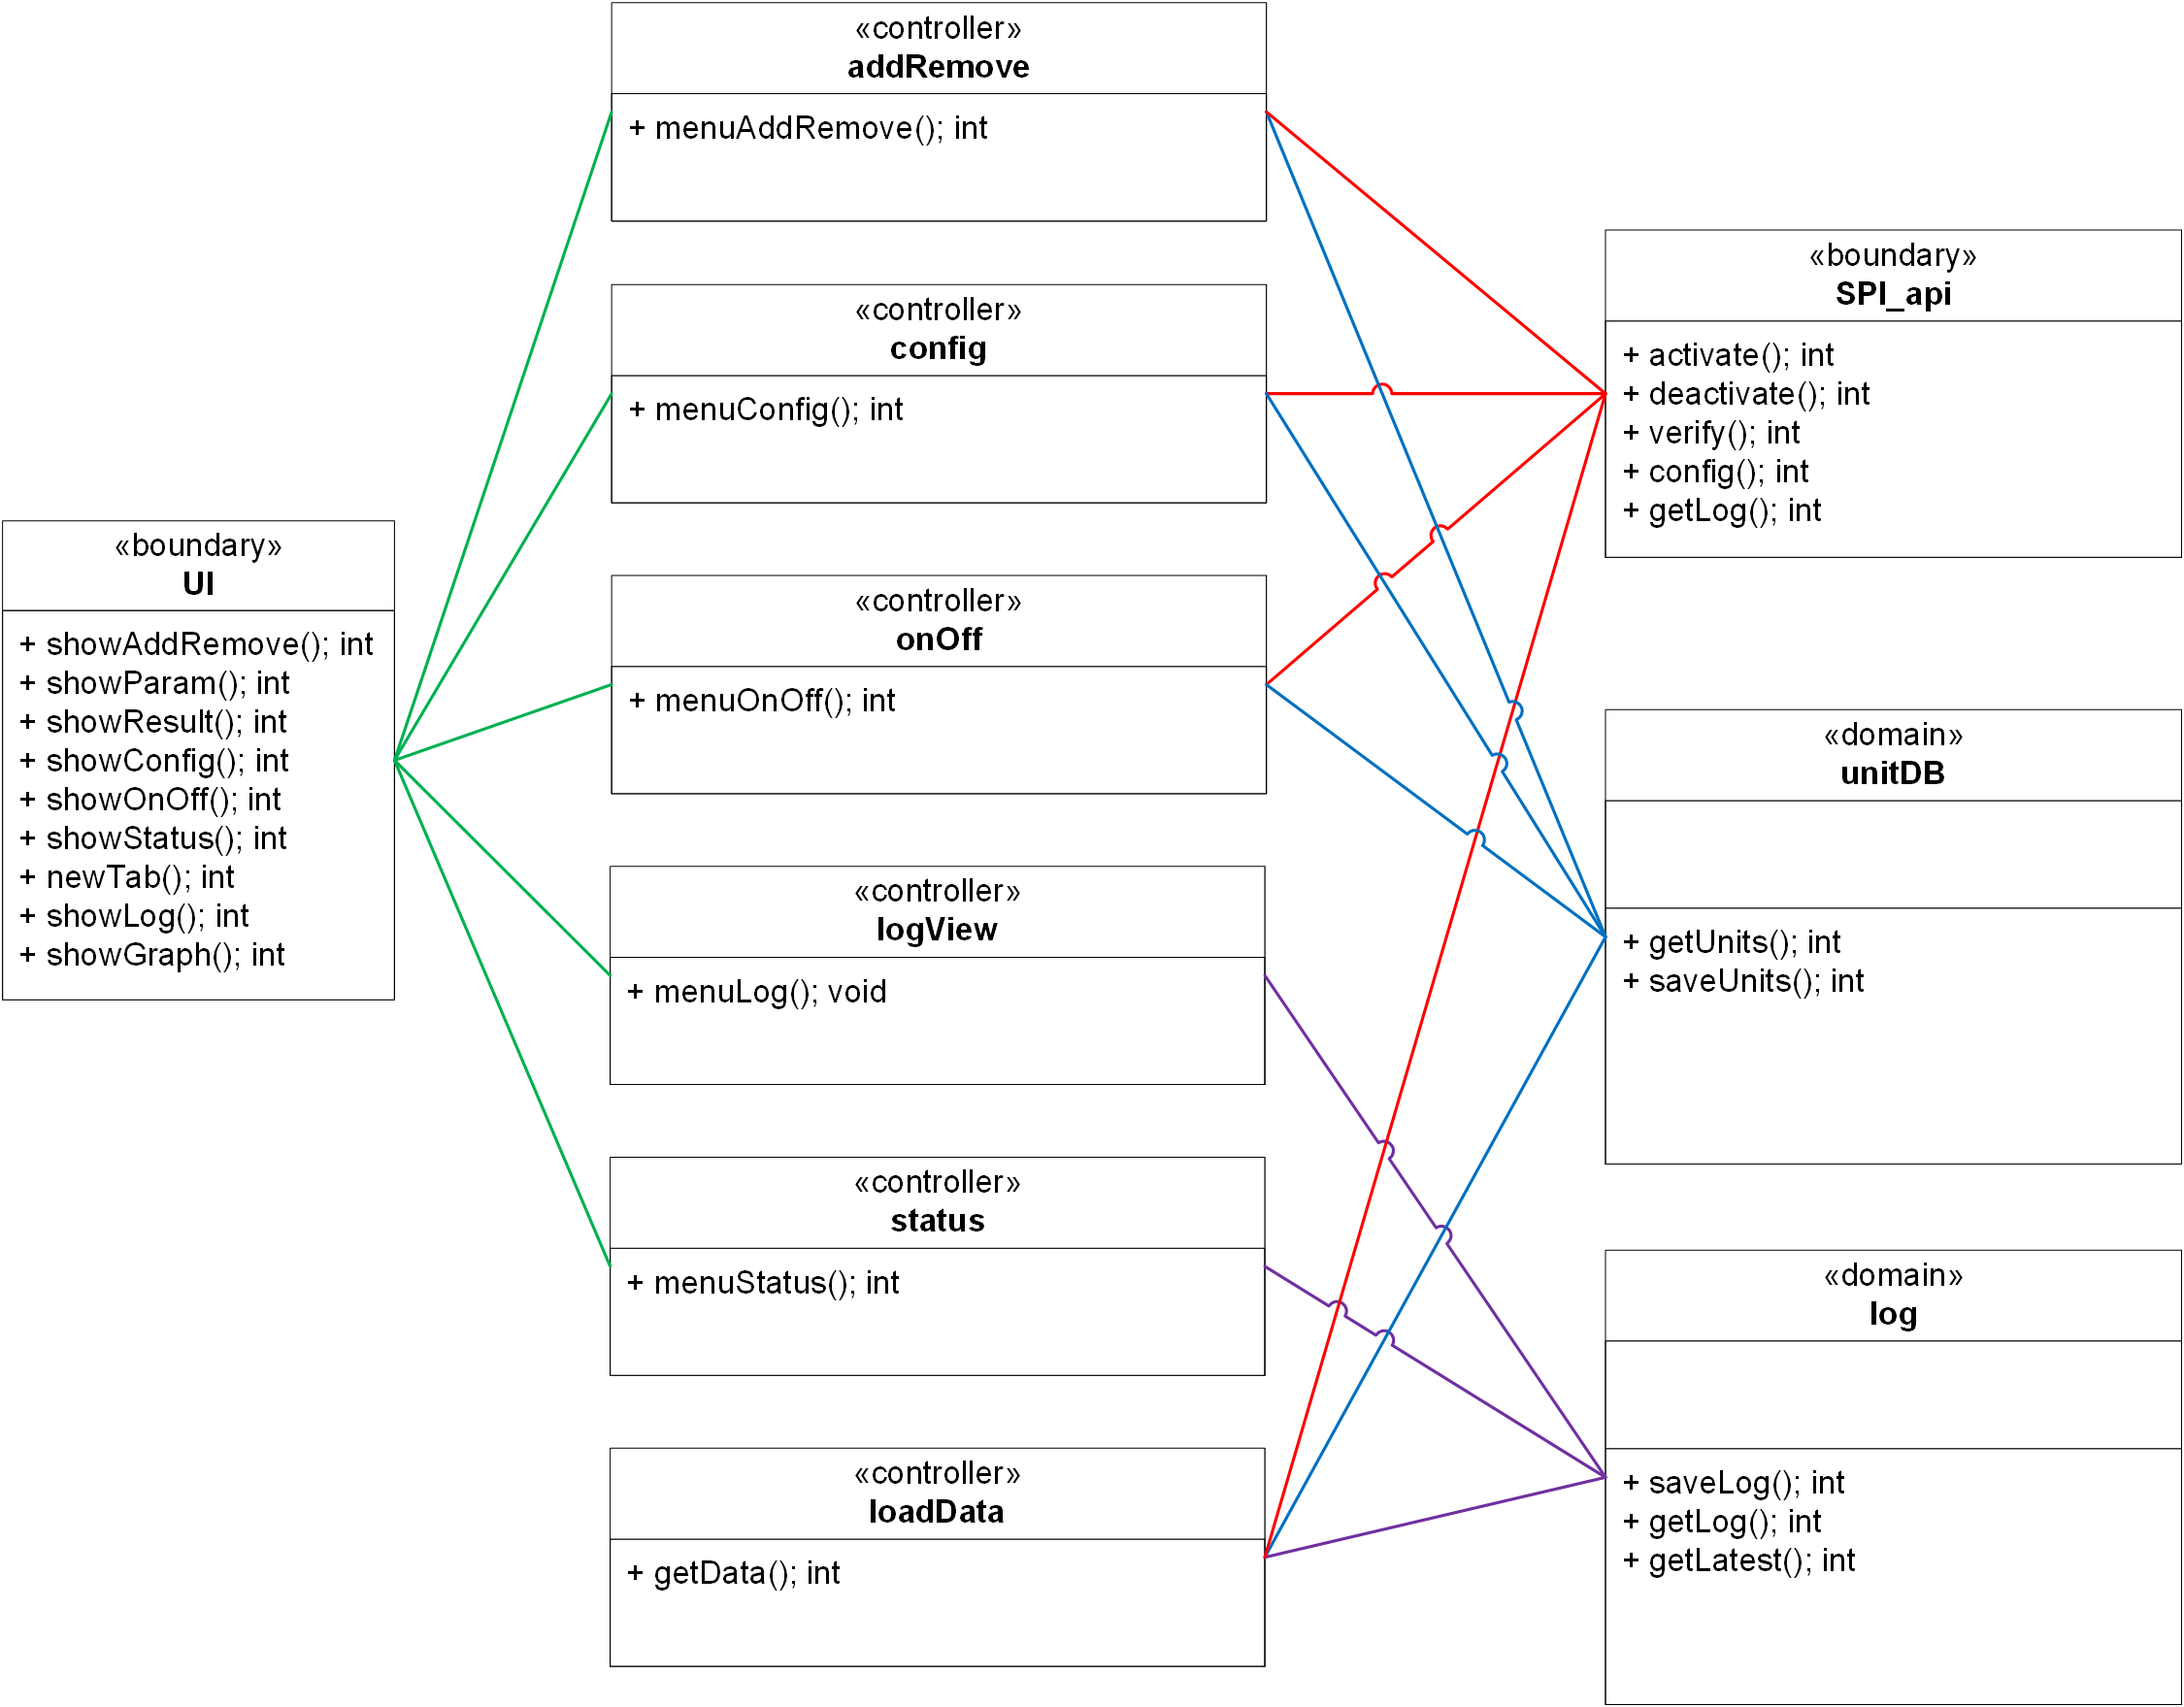
\includegraphics[scale=1]{filer/design/sw_class_devkit}}
\caption{klassediagram devkit8000}
\label{fig:klassediagram devkit8000}
\end{figure} 

Efter udarbejdelsen af sekvensdiagrammer samles alle metode kald imellem klasserne til et klassediagram som ses ovenfor på \ref{fig:klassediagram devkit8000}. Efter dette klassediagram udarbejdes en klassebeskrivelse hvor der tænkes over hvilke attributer de forskellige metoder skal have for at kunne udføre deres ansvar. Det bliver så fuldt op med et endeligt statisk klassediagram som inkludere alle attributer og medlems data.


\clearpage
\subsection{Enhed}
Applikationsmodeller for Enhed.